\chapter{Aproximaci{\'o}n de ra{\'i}ces}
    \section{Introducción}
    \justifying 
    En este capítulo se desarrollarán métodos numéricos para aproximar las soluciones (reales) de ecuaciones del tipo $f(x)=0$. La motivación de estos métodos es la necesidad de determinar la expresión en base decimal de las soluciones de una ecuación cuando dichas soluciones no son números racionales. 

    La forma de construir la mayoría de métodos será a partir de sucesiones de números racionales que convergerán a la solución de $f(x)=0$ ya que, por definición, todo número real es el límite de una sucesión de Cauchy de números racionales.

    Algo a tener en cuenta a la hora de emplear un método numérico es el error cometido. Como es imposible conocer el valor exacto del error (ya que entonces sabríamos cuál es la solución exacta), lo que haremos será acotar dichos errores. 
    \section{Algoritmo babilónico}
    \begin{ejem}
    
    Considerando la ecuación $x^2-2=0$, las soluciones son $x=\pm \sqrt{2}$, pero queremos saber la solución exacta (en el sentido numérico). Para ello, podemos generar una sucesión que converja a ella y que lo haga lo suficientemente rápido. 

    Consideremos la aproximación $x_o=1,5$, observemos que $\dfrac{2}{x_o}< 2$ y haciendo la media de ellas, obtenemos la siguiente aproximación:
    $$x_1=\dfrac{1}{2}\left(x_o+\dfrac{2}{x_o}\right)=1,4166...$$
    y de la misma forma
    $$x_2=\dfrac{1}{2}\left(x_1+\dfrac{2}{x_1}\right)=1,41421686...$$
    y dado que $\sqrt{2}=1,414213...$, hemos obtenido un error mínimo en unas pocas iteraciones. Veamos ahora el caso general.
    \end{ejem}
    \begin{met}[\textbf{Algoritmo babilónico}]
    Sea $a>0$. Queremos aproximar $\alpha=\sqrt{a}>0$, es decir, la raíz positiva de la ecuación
    $$x^2-a=0$$
    Dado $x_o>\alpha$, definimos la siguiente sucesión de aproximaciones:
    \begin{align}
    x_n=\frac{1}{2}\left(x_{n-1}+\frac{a}{x_{n-1}}\right)\qquad n\geq 1
    \end{align}
    Que convergerá al valor $\alpha$ con error 
    $$\varepsilon_{n}\leq k \cdot \varepsilon_{n-1}^2$$
    \end{met}
    \begin{dem}
    Calculemos en primer lugar el error cometido en la $n-$ésima iteración:
    $$\varepsilon_n=x_n-\alpha=\frac{1}{2}\left(x_{n-1}+\frac{a}{x_{n-1}}\right)-\alpha=\frac{1}{2x_{n-1}}(x_{n-1}^2+a-2\alpha x_{n-1})=\frac{1}{2x_{n-1}}(x_{n-1}-\alpha)^2>0$$
    luego $x_n>\alpha$ y como $\varepsilon_{n-1}=x_{n-1}-\alpha$, se deduce que
    $$\varepsilon_n=\frac{1}{2x_{n-1}}\cdot \varepsilon_{n-1}^2\leq \frac{1}{2\alpha}\cdot \varepsilon_{n-1}^2=k\cdot \varepsilon_{n-1}^2$$
    Veamos la convergencia del método:
    $$x_{n+1}-x_n=\frac{1}{2}\left(x_n+\frac{a}{x_n}\right)-x_n=\frac{1}{2x_n} \: a-\frac{1}{2} \: x_n=\frac{1}{2x_n}(a-x_n^2)=\frac{1}{2x_n}(\alpha-x_n)(\alpha+x_n)<0$$
    Como la sucesión es decreciente y acotada ($x_n>\alpha$) sabemos que converge. Tomando límites en $(1)$ y denotando por $\ell$ a dicho límite, obtenemos la siguiente ecuación:
    $$\ell=\frac{1}{2}\left(\ell+\frac{a}{\ell}\right)\Longrightarrow 2\ell^2=\ell^2+a\Longrightarrow \ell=\sqrt{a}=\alpha$$
    \qed\end{dem} 
    \begin{obs}
    El hecho de que el error en la iteración $n-$ésima esté acotado por el error de la iteración anterior al cuadrado indica que en cada aproximación el número de decimales que coinciden con el valor real se duplica. Esto se puede observar en el primer ejemplo.
    \end{obs}
    \section{{\'O}rdenes de convergencia} 
    \begin{defin}
        Sea $\{x_n\}$ una sucesión convergente con límite $L$, diremos que $\{x_n\}$  tiene un \textbf{orden de convergencia lineal} si 
        $$|x_{n+1}-L|\leq k \cdot |x_n-L| \qquad k <1$$
        Diremos que la sucesión $\{x_n\}$ tiene un \textbf{orden de convergencia cuadrática} si 
        $$|x_{n+1}-L|\leq k \cdot |x_n-L|^2 $$
        En general, diremos que la convergencia de $\{x_n\}$ es de \textbf{orden }$\mathbf{a}$ si
        $$|x_{n+1}-L|\leq k \cdot |x_n-L|^a $$
        El caso $1<a<2$ se denomina convergencia \textbf{superlineal}.
    \end{defin}

    \begin{obs}
    Equivalentemente, podemos definir los ordenes de convergencia como sigue.  Sea $\{x_n\}$ una sucesión convergente con límite $L$, diremos que la convergencia es lineal o de orden 1 cuando
        $$\lim_{n \to \infty} \dfrac{|x_{n+1}-L|}{|x_n-L|}=k < 1$$
        En general, la convergencia es de orden $a>1$ cuando 
        $$0 < \lim_{n \to \infty} \dfrac{|x_{n+1}-L|}{|x_n-L|^a}=k < +\infty$$

    \end{obs}
    
\section{M{\'e}todo de la bisecci{\'o}n}
        
       \begin{prop}
        Sea $f: \mathbb{R} \longrightarrow \mathbb{R}$ una función real de variable real. Si $f$ es continua en $I \subset \mathbb{R}$ y $f(a) \cdot f(b) < 0$ para $a < b \in I$ entonces existe $\alpha \in (a,b)$ tal que $f(\alpha)=0$. Además, si $f$ es derivable en $I$ y $f'(x) \neq 0 \: \forall x \in (a,b)$, entonces $\alpha$ es única.           
           \end{prop}
\begin{dem}
Como $f$ es continua en $[a,b]$, aplicando el teorema de Bolzano sabemos que existe $\alpha\in(a,b)$ tal que $f(\alpha)=0$. Por el teorema de Rolle, si existieran $\alpha_1,\alpha_2$ tales que $f(\alpha_1)=f(\alpha_2)=0$ existiría un punto $c\in (\alpha_1,\alpha_2)\subset(a,b)$ tal que $f'(c)=0$, lo cual contradice lo supuesto.
\qed\end{dem}
\begin{met}[\textbf{de la bisección}]
Sea $a<b$, $x_o=a$,  $y_o=b$ y $z_o=\frac{1}{2}(x_o+y_o)$. Queremos aproximar la solución de la ecuación $f(x)=0$. Si $f(a)\cdot f(b)<0$, por la proposición anterior sabemos que existe $\alpha\in(a,b)$ tal que $f(\alpha)=0$. Con lo cual: \vspace{-5mm}
\begin{itemize}
\item Si $f(z_o)=0$, entonces $\alpha=z_o$ es la solución.
\item Si $f(z_o) \neq 0$, tenemos dos opciones,
\begin{itemize}
    \item Si $f(x_o) \cdot f(z_o) < 0$, entonces tomamos $x_1=x_o, \: y_1=z_o,\: z_1=\frac{1}{2}(x_1+y_1)$
    \item Si $f(x_o) \cdot f(z_o)>0$, entonces tomamos $x_1=z_o, \: y_1=y_o,\: z_1=\frac{1}{2}(x_1+y_1)$
\end{itemize}
\end{itemize}
Aplicando la proposición anterior en $(x_1,y_1)$ nos aseguramos de que $\alpha\in(x_1,y_1)$. Reiterando este proceso, construimos tres sucesiones $\{x_n\}, \: \{z_n\}, \: \{y_n\}$ tales que $x_n\leq z_n\leq y_n$. Observemos además que
\begin{enumerate}[a)]
    \item $\{x_n\}$ es una sucesión creciente y acotada (superiormente) por $\{y_n\}$ 
    
    \item $\{y_n\}$ es una sucesión decreciente y acotada (inferiormente) por $\{x_n\}$

Luego ambas sucesiones son convergentes. Denotemos por $\alpha,\beta$ a los límites de $\{x_n\}$ e $\{y_n\}$ respectivamente. Se tiene entonces que:
$$\beta-\alpha=\underset{n\to\infty}{\lim}(y_n-x_n)=\underset{n\to\infty}{\lim}\frac{b-a}{2^n}=0$$
\item  Como $f$ es continua, $\{f(x_n)\}$ es una sucesión convergente (análogamente $f(\{y_n\})$). Además,  \vspace{-3mm}
$$f(x_n) \cdot f(y_n) <0 \: \Rightarrow \:  \lim_{n \to \infty} f(x_n) \cdot f(y_n) \leq 0 \: \Rightarrow \: \lim_{n \to \infty} f(x_n)  \lim_{n \to \infty} f(y_n) =f(\alpha)^2\leq 0$$
por tanto, $f(\alpha)=0.$
\end{enumerate}
Estudiemos ahora el error del método. Sea $\{z_n\}$ la sucesión que obtenemos por el método de la bisección, y sea 
$$\varepsilon_n=z_n - \alpha$$
el error en el término $n$, entonces, por lo visto en b),
$$|\: \varepsilon_n|=|z_n - \alpha|< \dfrac{b-a}{2^{n+1}}$$
De esta manera, si queremos aproximar $\alpha$ con un error (en valor absoluto) menor que $\varepsilon$, tendrá que ser 
$$|\varepsilon_n|=\dfrac{b-a}{2^{n+1}} < \varepsilon \iff 2^{n+1} > \dfrac{b-a}{\varepsilon} \iff (n+1) \log(2) > \log(b-a) - \log(\varepsilon) $$
Es decir, $$n > \dfrac{\log(b-a)-\log(\varepsilon)}{\log(2)}-1$$
para el $\varepsilon$ que se quiera elegir.
\end{met}
\begin{intgraf} Podemos ver un ejemplo de este método con la siguiente figura, donde escogemos $\alpha \in [a,b]$ ya que $\alpha\approx 1.41$ y $[a,b]=[0'7,1'8]$, y hacemos un par de iteraciones, observando como acotamos la raíz, pero la convergencia no es óptima.
$$\begin{tikzpicture}[scale=3, domain=-1:2, samples=70,  trig format=rad]
    
	% draw axis
	\draw[->] (-0.3,0) -- (3,0) node[below right] {$x$};
	\draw[->] (0,-0.5) -- (0,1.3) node[above left] {$y$};
	
	% draw function
	\draw[blue, thick] plot[domain=0.2:2.2] (\x,0.33*\x*\x-0.5) node[above right] {\footnotesize $f(x)=x^2-4$};

    \draw[fill=black] (1.23,0) circle [radius=0.01] node[above] {$\alpha$};
     \draw[fill=black] (0.7,0) circle [radius=0.01] node[above] {$a=x_o=x_1$ \hspace{15mm}};
     \draw[fill=black] (2,0) circle [radius=0.01] node[below right] {$b=y_o$ \; \; };
     \draw[dotted] (2,0) -- (2,0.82);
     \draw[dotted] (0.7,0) -- (0.7,-0.34);
     \draw[fill=black] (1.35,0) circle [radius=0.01] node[below right] {$z_o=y_1\; \; \; \;$};
     \draw[<-] (1.025,-0.01) -- (1.2,-0.3)  node[below] {$\; \; \; z_1$};
     \draw[->] (1.025,0) circle [radius=0.01];
     
\end{tikzpicture}$$    
\end{intgraf}
\begin{ejem}
    Escogiendo $\varepsilon=10^{-8}$, para hallar $\sqrt{2}$ y eligiendo $a=1, \: b=2$, $$n>\dfrac{\log(1)-\log(10^{-8})}{\log(2)}=\dfrac{8\log(10)}{\log(2)} = 8 \cdot \log_2(10) > 26$$
    Es decir, hacemos más de 26 iteraciones, que comparadas con las 3-4 que necesitábamos con el método babilónico, nos da un método mucho más lento.
\end{ejem}
\begin{obs}\:\vspace{-5mm}
    \begin{enumerate}[a)]
        \item No se calcula el producto $f(x_n)\cdot f(z_n)$, solo se mira el signo de $f(z_n)$
        \item No se calcula $z_o=\dfrac{1}{2}(x_o+y_o)$, sino 
        $$z_o=x_o+\dfrac{\Delta_o}{2} \quad \Delta_o=y_o-x_o$$
        teniendo así en $\Delta_i$ el error de la iteración $i$.
    \end{enumerate}
\end{obs}
    \section{M{\'e}todo del punto fijo}
       \begin{defin}
           Un \textbf{punto fijo} de una aplicación
           $g$ es aquel tal que $$g(\alpha)=\alpha$$
           En el caso de funciones $g: \mathbb{R} \longrightarrow \mathbb{R}$, se trata de encontrar la solución de la ecuación $g(x)=x$.
       \end{defin}
       \begin{teo}[\textbf{del punto fijo de Brower}] Si $f: [a,b] \longrightarrow [a,b]$ con $a,b \in \mathbb{R}$ es continua, entonces $f$ tiene un punto fijo, $\alpha\in[a,b]$.
       \end{teo}
       \begin{dem}
           El caso $f(a)=a$ ó $f(b)=b$ es trivial. Si $f(a)\neq a$, entonces $f(a)>a$, luego $f(a)-a>0$, y de la misma forma, $f(b)-b <0$. Como la función $g(x)=f(x)-x$ es continua, por el Teorema de Bolzano, existe $\alpha \in (a,b)$ tal que $$0=g(\alpha)=f(\alpha)-\alpha \: \iff \: f(\alpha)=\alpha$$ 
       \qed\end{dem}
       \begin{defin}
           Una función $f$ se dice que es \textbf{contractiva} cuando existe una constante $k < 1$ tal que
           $$|f(x)-f(y)| \leq k \cdot |x-y|$$
       \end{defin}
       \begin{defin}
       Las funciones que verifican $$|f(x)-f(y)|\leq L \cdot |x-y|$$ para cierta $L \in \mathbb{R}$ se llaman \textbf{funciones lipschitzianas}.
       \end{defin}
       \begin{teo} [\textbf{del punto fijo de Banach}] Si $f: [a,b] \longrightarrow [a,b]$ es contractiva, entonces $f$ tiene un único punto fijo. 
       \end{teo}
       \begin{dem}
           Por ser $f$ contractiva, es continua y aplicando el Teorema del Punto Fijo de Brower, tiene un punto fijo. Veamos que el punto fijo es único. Supongamos que existen dos distintos, $\alpha, \beta$, entonces sería
           $$|\alpha-\beta|=|f(\alpha)-f(\beta)| \leq k \cdot |\alpha-\beta| < \alpha-\beta$$
           lo cual es una contradicción, luego existe un único punto fijo.
       \qed\end{dem}
       \begin{ejer}
       Si $f: \mathbb{R} \longrightarrow \mathbb{R}$ es contractiva, entonces $f$ tiene un único punto fijo.
       \end{ejer}
       \begin{met}[\textbf{del punto fijo}] Si $f$ es una aplicación contractiva en un entorno $I$ de un punto fijo $\alpha$, entonces para todo $x_o \in I$, la sucesión
       \begin{align}
           x_{n+1}=f(x_n) \qquad n \geq 0
           \label{met:punto}
        \end{align}
           converge a $\alpha$ con un orden de convergencia lineal:
           $$|\varepsilon_n|\leq k |\varepsilon_{n-1}| \qquad k<1$$
       \end{met}
       \begin{dem}
       Veamos en primer lugar que la sucesión converge a $\alpha$:
           $$|x_{n+1}- \alpha|=|f(x_{n})-f(\alpha)|\leq k \cdot |x_n - \alpha|\leq k^2 \cdot |x_{n-1}- \alpha| \leq \cdots \leq k^{n+1} \cdot |x_o - \alpha|$$
Como $\underset{n \to \infty}{\lim} k^n=0$, dado $\varepsilon>0$ existe $n_o \in \mathbb{N}$ tal que para todo $n > n_o$, $k^{n+1} < \frac{\varepsilon}{|x_o-\alpha|}$, de forma que para todo $n>n_o$ se verifica que
$$|x_{n+1}-\alpha|<k^{n+1}\cdot |x_o-\alpha|<\frac{\varepsilon}{|x_o-\alpha|}\cdot |x_o-\alpha| <\varepsilon$$
Estudiemos ahora el error. El error cometido en la $n$-ésima iteración será $|\varepsilon_n|=|x_n-\alpha|$ y por ser $f$ contractiva se tiene que
$$|\varepsilon_{n}|=|x_{n}-\alpha|=|f(x_{n-1})-f(\alpha)|\leq k \cdot |x_{n-1} - \alpha| = k \cdot |\varepsilon_{n-1}|$$
            Es decir, el método del punto fijo tiene un orden de convergencia lineal.
       \qed\end{dem} 
       \begin{intgraf} Podemos ver a continuación un ejemplo del método, donde observamos como nos vamos enroscando sobre el punto fijo $\alpha$ de $\cos(x)$, que como se puede observar debajo, es la solución o raíz de $\cos(x)-x$, que hemos llamado $\beta$.
$$\begin{tikzpicture}[scale=5, domain=-1:2, samples=70,  trig format=rad]
	
	% draw axis
	\draw[->] (-0.3,0) -- (2,0) node[below right] {$x$};
	\draw[->] (0,-0.5) -- (0,1.3) node[above left] {$y$};
	
	% draw function
	\draw[blue, thick] plot[domain=-0.1:2] (\x,{cos(\x)}) node[above right] {\footnotesize $f(x)=\cos(x)$};
    \draw[blue, thick] plot[domain=-0.1:1.2] (\x,{(\x)}) node[right] {\footnotesize $f(x)=x$};
    \draw[black, thick] plot[domain=-0.1:1] (\x,{cos(\x)-\x}) node[right] {\footnotesize $f(x)=\cos(x)-x$};

    \draw[fill=black] (0.74,0.74) circle [radius=0.01] node[above] {$\alpha$};
    \draw[fill=black] (0.74,0) circle [radius=0.01] node[below] {$\beta$};
    \draw[dotted] (0.74,0.74) -- (0.74,0);
    \def\x{1}
    \draw[fill=black] (\x,0) circle [radius=0.01] node[below] {$x_o$};
    \draw[dotted] (\x,0) -- (\x,{cos(\x)});
    \def\y{0.54}
    \draw[fill=black] (\y,0) circle [radius=0.01] node[below] {$x_1$};
    \draw[dotted] (\y,0) -- (\y,\y);
    \draw[red,fill=red] (\x,{cos(\x)}) circle [radius=0.01];
    \draw[->,red](\x,{cos(\x)}) -- (\y,\y) ;
    \draw[dotted] (\y,0) -- (\y,{cos(\y)}); 
    \draw[->,red](\y,\y) -- (\y,{cos(\y)});

    \def\z{0.86}
    \draw[fill=black](\z,0) circle [radius=0.01] node[below] {$x_2$};
    \draw[dotted] (\z,0) -- (\z,\z);
    \draw[->,red] (\y,{cos(\y)}) -- (\z,\z);
    \draw[red,->] (\z,\z) -- (\z,{cos(\z)});

    \def\t{0.65}
    \draw[fill=black](\t,0) circle [radius=0.01] node[below] {$x_3$};
    \draw[dotted] (\t,0) -- (\t,\t);
    \draw[->,red] (\z,{cos(\z)}) -- (\t,\t);
    \draw[red,->] (\t,\t) -- (\t,{cos(\t)});

    
\end{tikzpicture}$$
       \end{intgraf}
       \begin{ejem}
           El algoritmo babilónico
           $$x_{n+1}=\dfrac{1}{2}\left( x_n + \dfrac{a}{x_n}\right)$$
           aproxima el punto fijo de $g(x)=\frac{1}{2}\left( x + \frac{a}{x}\right)$, es decir, solución de $g(x)=x$ $$x=\frac{1}{2}\left( x + \frac{a}{x}\right) \iff 2x=x+\dfrac{a}{x} \iff x = \dfrac{a}{x} \iff x^2=a$$
           Veamos que $g$ es contractiva en un entorno de $\alpha=\sqrt{a}$. Dado que la contractividad asegura que $$\dfrac{|g(x)-g(y)|}{|x-y|}\leq k <1$$
           Si $g$ es drivable (que lo es en nuestro ejemplo), aplicando el teorema del valor medio tenemos que 
           $$\dfrac{|g(x)-g(y)|}{|x-y|}=|g'(\xi)| \qquad \xi \in (x,y)$$
           Por tanto, si $g'$ es continua en un entorno de $\alpha$ y $|g'(\alpha)|<1$, entonces $|g'(x)|\leq k <1$ en un entorno de $\alpha$. En nuestro caso, $g'(x)=\frac{1}{2}\left(1-\frac{a}{x^2}\right)$, es decir, $g'(\alpha)=g'(\sqrt{a})=0$, luego $|g'(x)|\leq k < 1$
       \end{ejem}
    
    \section{M{\'e}todo de Newton}          
    \begin{teo}[\textbf{de Taylor}]
    Dada $f \in \mc{C}^{n+1}$, se verifica que
    $$f(b)=\sum_{k=0}^n \dfrac{f^{(k)}(a)}{k!}(b-a)^k + R_k(a)$$
    Donde el resto $R_k(a)$ toma las formas de Lagrange e integral
    $$R_k(a)=\dfrac{f^{n+1}(\xi)}{(n+1)!}(b-a)^{n+1} = \dfrac{1}{n!} \int_0^1 f(x) (b-x)^n dx$$
    \end{teo}
    \begin{obs}
        Sea $f: \mathbb{R} \longrightarrow \mathbb{R}$ una función derivable con $f(\alpha)=0$. Una primera aproximación a $\alpha$ es la siguiente:
 
        Dado $x_o$, aproximamos la curva $y=f(x)$ por la tangente en $x=x_o$. La ecuación de la recta tangente es $y=f(x_o)+f'(x_o)(x-x_o)$ de manera que el corte con $y=0$ es:
        $$x_1=x_o-\dfrac{f(x_o)}{f'(x_o)}$$
    \end{obs}
    \begin{met}[\textbf{de Newton}]
        Sea $f$ una función de clase $\mc{C}^2(I)$ con $I \subset \mathbb R$ y sea $\alpha \in I$ tal que $f(\alpha)=0, \: f'(\alpha)\neq 0$. Entonces la sucesión $\{x_n\}$ definida por 
        \begin{align}
          x_{n+1}=x_n-\dfrac{f(x_n)}{f'(x_n)} \qquad n \geq 0
          \label{met:newton}
        \end{align}
        
        coverge a $\alpha$ para $x_o \in I$ suficientemente próximo a $\alpha$. Ademas, dicha convergencia será cuadrática:
        $$|x_{n+1}-\alpha|< C \: |x_n-\alpha|^2 \qquad C=\dfrac{\max|f''(x)|}{2\min|f'(x)|} $$
    \end{met}
    \begin{dem}
        Considerando la función $g(x)=x-\frac{f(x)}{f'(x)}$, observemos que $$g(\alpha)=\alpha-\dfrac{\cancelto{0}{f(\alpha)}}{f'(\alpha)}=\alpha$$es decir, $\alpha$ es un punto fijo de $g$. Si $g$ es contractiva en un entorno de $\alpha$, concluiríamos por la convergencia del punto fijo.

        Calculamos entonces que
        $$g'(x)=1- \dfrac{f'(x)}{f'(x)}+f(x) \: \dfrac{f''(x)}{f'(x)^2}=f(x)\dfrac{f''(x)}{f'(x)^2}$$
        por lo que $$g'(\alpha)=f(\alpha) \: \dfrac{f''(\alpha)}{f'(\alpha)^2}=0$$
        
        Como $g'$ es continua en $\alpha$, dado cualquier $\varepsilon > 0$, podemos encontrar $\delta > 0$ tal que si $|x-\alpha| < \delta$, $$|g'(x)-g'(\alpha)|< \varepsilon \iff |g'(x)|< \varepsilon$$

        Es decir, dado $0 < k < 1$, tomando $\varepsilon=k$ podemos encontrar un $\delta > 0$ tal que si $x \in (\alpha- \delta, \alpha+\delta)$, entonces $|g'(x)| < k$. Dados $x_1,x_2\in(\alpha-\delta,\alpha+\delta)$, por el teorema del valor medio se tiene que
        $$\dfrac{|g(x_1)-g(x_2)|}{|x_1-x_2|}=|g'(\xi)|<k\Rightarrow |g(x_1)-g(x_2)|<k\cdot |x_1-x_2|$$
        y, por tanto, $g$ es contractiva en $(\alpha- \delta, \alpha+\delta)$.
        
        Estudiemos ahora el error del método:
    $$x_{n+1}-\alpha=x_n-\dfrac{f(x_n)}{f'(x_n)} - \alpha=\dfrac{1}{f'(x_n)}(f'(x_n)(x_n-\alpha)-f(x_n))$$
    De la fórmula de Taylor de primer orden se tiene que
    $$0=f(\alpha)=f(x_n)+f'(x_n)(\alpha-x_n)+\dfrac{1}{2}f''(\xi)(\alpha-x_n)^2=f(x_n)-f'(x_n)(x_n-\alpha)+\dfrac{1}{2}f''(\xi)(x_n-\alpha)^2$$
    Por tanto, se tiene que 
    $$x_{n+1}-\alpha=\dfrac{1}{f'(x_n)}f''(\xi)(x_n-\alpha)^2$$
    De esta manera, $$|x_{n+1}-\alpha|=\dfrac{|f''(\xi)|}{2|f'(x_n)|}\: |x_n-\alpha|^2 < \dfrac{\max|f''(x)|}{2\min|f'(x)|}\: |x_n-\alpha|^2 \qquad x \in I$$
    Es decir,
    $$|x_{n+1}-\alpha|< C \: |x_n-\alpha|^2 \qquad C=\dfrac{\max|f''(x)|}{2\min|f'(x)|} $$
    Obteniendo así una convergencia cuadrática.
    \qed\end{dem}
    \begin{intgraf} Véanse las siguientes figuras, una de la $n$-ésima iteración del método de Newton, escogiendo como $x_{n+1}$ el corte de la tangente que pasa por $f(x_n)$, y un ejemplo en el que el método no converge:
    $$\begin{tikzpicture}[scale=2.5, domain=0.3:2, samples=50]
	
	% draw axis
	\draw[->] (-0.1,0) -- (2.5,0) node[below right] {$x$};
	\draw[->] (0,-0.5) -- (0,2.2) node[above left] {$y$};
	
	% draw function
	\draw[blue, thick] plot (\x, {0.5*\x*\x-0.2}) node[left] {\footnotesize $f(x)$};

	% draw x-axis intercept
    \def\x{1.6};
	\draw[dotted] (\x, 0) node[below] {\footnotesize $x_n$} -- (\x,{0.5*\x*\x-0.2});
    \draw[color=red]    plot (\x,1.543*\x-1.4);
    \draw[fill=black] (\x,{0.5*\x*\x-0.2}) circle [radius=0.018] node[left] {\footnotesize $f(x_n)$};
    \draw[fill=black] (\x,0) circle [radius=0.018];
    \draw[fill=black] (0.632,0) circle [radius=0.018] node[below] {\footnotesize $\alpha$};
 
    \def\x{0.9};
	\draw[dotted] (\x, 0) node[below right] {\footnotesize $x_{n+1}$} -- (\x,0.205);
	\draw[fill=black] (\x,0) circle [radius=0.018];
	
\end{tikzpicture}$$
\begin{center}
    Un ejemplo gráfico del Método de Newton en la función $y=\frac{1}{2} \: x^2-\nicefrac{1}{5}$
\end{center}
$$\begin{tikzpicture}[scale=1.5, domain=-1:1.4, trig format=rad, samples=100]
	% draw axis
	\draw[->] (-4,0) -- (4,0) node[right] {$x$};
    \draw[dashed] (-4,1.54) -- (4,1.54) node[right] {\footnotesize $\dfrac{\pi}{2}$};
    \draw[dashed] (-4,-1.54) -- (4,-1.54) node[right] {\footnotesize $-\dfrac{\pi}{2}$};
	% draw function
    \draw[blue,thick] plot[variable=\t,domain=-3:3.3] (\t,{atan(5*\t)}) node[below right] {\footnotesize $f(x)$};
	% draw x-axis intercept
    \def\x{0.4};
    \draw[dotted] (\x, 0) node[below] {\footnotesize $x_o$} -- (\x,{atan(5*\x)});
    \draw[fill=black] (\x,{atan(5*\x)}) circle [radius=0.03];
    \draw[fill=black] (\x,0) circle [radius=0.03];

    \draw[fill=black] (0,0) circle [radius=0.03] node[above left] {\footnotesize $\alpha$};
    \def\x{3};
	\draw[dotted] (\x, 0) node[below right] {\footnotesize $x_2$} -- (\x,{atan(5*\x)});
    \draw[fill=black] (\x,{atan(5*\x)}) circle [radius=0.03];
    \draw[<-,color=red,thick]  (-0.8,0) -- (0.4,{atan(5*0.4)})  ;
    \draw[fill=black] (\x,0) circle [radius=0.03];
    
    \def\x{-0.8};
	\draw[dotted] (\x, 0) node[above left] {\footnotesize $x_1$} -- (\x,{atan(5*\x)});
    \draw[->,color=red,thick] (\x,{atan(5*(\x))}) -- (3,0) ;
    \draw[fill=black] (\x,0) circle [radius=0.03];
    \draw[fill=black] (-0.8,{atan(5*(-0.8))}) circle [radius=0.03];
	\draw[->,color=red,thick] (3,1.525) -- (-3,1.525) ;
\end{tikzpicture}$$
\begin{center}
    Un ejemplo del Método de Newton en el que no converge en la función $y=\arctan(x)$.
\end{center}
    \end{intgraf}
    \begin{ejem}
        Consideremos $f(x)=x^2-a$. Dado $x_o$, el método de Newton para esta ecuación es
        $$x_{n+1}=x_n-\dfrac{f(x_n)}{f'(x_n)}=x_n-\dfrac{x_n^2-a}{2x_n}=\dfrac{2x_n^2-x_n^2+a}{2x_n}=\dfrac{x_n^2+a}{2x_n}=\dfrac{1}{2}\left(x_n+\dfrac{a}{x_n}\right)$$
        Es decir, el método babilónico es el método de Newton aplicado a dicha $f(x)$.
    \end{ejem}
    \begin{ejem}
        Considerando ahora $f(x)=x^3-a$, el método de Newton sería
        $$x_{n+1}=x_n-\dfrac{f(x_n)}{f'(x_n)}=x_n-\dfrac{x_n^3-a}{3x_n^2}=\dfrac{3x_n^3-x_n^3+a}{3x_n^2}=\dfrac{1}{3} \left( 2x_n + \dfrac{a}{x_n^2}\right)$$
    \end{ejem}
    \begin{obs}
        Ahora bien, no sabemos cuan cerca de $\alpha$ estamos, por lo que vamos a buscar un $x_o$ adecuado. Por ejemplo, en el caso de una aplicación con punto de inflexión (cambia su concavidad), puede pasar que el método no converja por ser $x_1=x_o$. 
    \end{obs}
    \begin{prop}
        Por tanto, supongamos que $f'(x)\neq 0$ y $f''(x)\neq 0$ en $x \in I$ donde $I$ es un intervalo que contiene a la solución. Si $x_o \in I$ verifica que $f(x_o) \cdot f''(x_o) > 0$, entonces el método de Newton converge.
    \end{prop}
        \begin{dem}
            Sabemos que $f'(x)\neq 0$, entonces para saber si $x_1$ está del mismo lado que $x_o$ o no (con respecto de $\alpha$), basta con ver el signo de $f(x_1)$, por ser $f$ monótona (creciente o decreciente). En efecto, 
            $$f(x_1)=f(x_o)+f'(x_o)(x_1-x_o)+\dfrac{1}{2}f''(\xi)(x_1-x_o)^2=\cancel{f(x_o)}+\cancel{f'(x_o)}\left(\dfrac{\cancel{-f(x_o)}}{\cancel{f'(x_o)}} \right)+\dfrac{1}{2}f''(\xi)(x_1-x_o)^2$$
            $$\Rightarrow \: f(x_1)=\dfrac{1}{2}f''(\xi)(x_1-x_o)^2$$
            Luego 
            $$sign \: f(x_1)=sign \: f''(\xi)=sign \: f''(x_o)=sign \: f(x_o)$$
            por la hipótesis de $f(x_o) \cdot f''(x_o) > 0$. Por tanto, se puede concluir que $x_o$ y $x_1$ están del mismo lado respecto de $\alpha$. Veamos pues que, usando Taylor, 
            $$x_1-x_o=-\dfrac{f(x_o)}{f'(x_o)}=-\dfrac{f(\alpha)+f'(\sigma)(x_o-\alpha)}{f'(x_o)}=- \dfrac{f'(\sigma)}{f'(x_o)}(x_o-\alpha)$$
            Como $f'(\sigma)$ y $f'(x_o)$ tienen el mismo signo, es 
            $$sign (x_1-x_o)=-sign (x_o-\alpha)=sign (\alpha-x_o)$$
            Por tanto, $x_1$ siempre está más para el lado de $\alpha$ que $x_o$ ($x_1$ está siempre entre $x_o$ y $\alpha$).

            Repitiendo este argumento construimos una sucesión $\{x_n\}$, creciente (si $x_o<\alpha$) o decreciente (si $x_o > \alpha$) y acotada, que es convergente con límite $\alpha$. 
        \qed\end{dem}
    
    \begin{ejem}
        Con $f(x)=x^2-a$, elegíamos siempre $x_o > \alpha$, $f''(x)=2x>0$. En cambio, eligiendo un $x_o$ más alla de $\sqrt{a}$, el método tarda más, pero finalmente, dado que $f(x)$ es ``tranquila'', converge.

        Dado $f(x_1)=f(\alpha)+\dfrac{1}{2}f''(\xi)(x_1-\alpha)^2$, esto implica que $$x_1-\alpha=\dfrac{f(x_1)}{f''(\xi)}$$
    \end{ejem}

    \subsection{Ra{\'i}ces m{\'u}ltiples}
    Dado que en todo momento hemos estado en la hipótesis de que $f'(\alpha)\neq 0$, nos preguntamos si necesitamos que se verifique necesariamente. Veamos que no, y que converge más lentamente en dicho caso.
    \begin{defin}
        Sea $f$ una función $n$ veces derivable en $\alpha$ tal que $f(\alpha)=f'(\alpha)= \: \cdots \: = f^{n-1}(\alpha)=0$, $f^n(\alpha)\neq 0$, entonces se dice que $\alpha$ es una \textbf{raíz de $f$ de multiplicidad $n$}.
    \end{defin}
    \begin{prop}
        Si $\alpha$ es una raíz de multiplicidad 2 o raíz doble, el método de Newton converge linealmente.
    \end{prop}
    \begin{dem}
        Siguiendo el mismo método que antes, 
        $$x_{n+1}-\alpha=x_n-\dfrac{f(x_n)}{f'(x_n)}=\dfrac{1}{f'(x_n)}(f'(x_n)(x_n-\alpha)-f(x_n))$$
        Haciendo ahora un término más de Taylor:
        $$f(x_n)=\cancelto{0}{f(\alpha)}+\cancelto{0}{f'(\alpha)}(x_n-\alpha)+\dfrac{1}{2}f''(\xi)(x_n-\alpha)^2$$
        $$f'(x_n)= \cancelto{0}{f'(\alpha)}+f''(\sigma)(x_n-\alpha)$$
        por tanto, sustituyendo arriba, tendríamos que 
        $$x_{n+1}-\alpha=\dfrac{1}{f''(\sigma)\cancel{(x_n-\alpha)}}\:(f''(\sigma)\cancel{(x_n-\alpha)}(x_n-\alpha)-\dfrac{1}{2}f''(\xi)(x_n-\alpha)^{\cancel{2}} )=\left(1-\dfrac{1}{2} \: \dfrac{f''(\xi)}{f''(\sigma)}\right)(x_n-\alpha)$$
        De forma que 
        $$|x_{n+1}-\alpha|\leq C \:|x_{n}-\alpha|$$ 
        Ya que
        $0<C=\left|1-\frac{f''(\xi)}{2f''(\sigma)}\right|\leq 1$
    \qed\end{dem}
  
    \begin{lem}
  Sea $f$ una función suficientemente derivable, $\mc{C}^{m+2}(I)$, y $\alpha$ una raíz de multiplicidad. Existe una función derivable $g(x)$ tal que 
$$f(x)=(x-\alpha)^m g(x) \; , g(\alpha) \neq 0$$
    \end{lem}
   \begin{dem}
        Por el desarrollo de Taylor,
        $$f(x)=\sum_{k=0}^m\dfrac{f^{(k)}(\alpha)}{k!}(x-\alpha)^k+\dfrac{f^{(m+1)}(\xi)}{(k+1)!}(x-\alpha)^{m+1}=$$
        $$=\dfrac{f^{(m)}(\alpha)}{m!}(x-\alpha)^m+\dfrac{f^{(m+1)}(\xi)}{(k+1)!}(x-\alpha)^{m+1}=(x-\alpha)^m\left(\frac{f^{(m)}(\alpha)}{m!}+\dfrac{f^{(m+1)}(\xi)}{(k+1)!}(x-\alpha)\right)=(x-\alpha)^m g(x)$$
        
        La función (inofensiva) $\frac{f(x)}{(x-\alpha)^m}$ es tan diferenciable como $f$ excepto (quizá) en $x=\alpha$. Para ello, dado que no está definida ahí, calcularemos su límite:
        $$\lim_{x \to \alpha}\dfrac{f(x)}{(x-\alpha)^m}\overset{L'H}{=}\lim_{x \to \alpha}\dfrac{f'(x)}{m(x-\alpha)^{m-1}}= \cdots = \lim_{x \to \alpha} \dfrac{f^{(m)}(x)}{m!}=\dfrac{f^{(m)}(\alpha)}{m!}$$
        Definimos entonces la función
        $$g(x)=\left\{\begin{array}{cc}
           \dfrac{f(x)}{(x-\alpha)^m}  & \text{ si } x\neq \alpha \\
           & \\
            \dfrac{f^{(m)}(\alpha)}{m!} & \text{ si } x=\alpha 
        \end{array}\right.$$
        que será continua por lo anteriormente demostrado. La función $g(x)$ es además derivable para todo $x \neq \alpha$. Estudiemos entonces el caso $x=\alpha$:
        $$\lim_{x\to \alpha}\dfrac{g(x)-g(\alpha)}{x-\alpha}=\lim_{x \to \alpha}\dfrac{\frac{f(x)}{(x-\alpha)^m}-\frac{f^{(m)}(\alpha)}{m!} }{x-\alpha}=\lim_{x \to \alpha}\dfrac{f(x)-\dfrac{f^{(m)}(\alpha)}{m!} (x-\alpha)^m}{(x-\alpha)^{m+1}}$$
        Lo cual, por el desarrollo de Taylor (expuesto al principio de la demostración)
        $$=\lim_{x\to\alpha}\dfrac{\frac{f^{(m+1)}(\xi)}{(m+1)!}\cancel{(x-\alpha)^{m+1}}}{\cancel{(x-\alpha)^{m+1}}}=\lim_{x\to\alpha}\frac{f^{(m+1)}(\xi)}{(m+1)!}=\frac{f^{(m+1)}(\alpha)}{(m+1)!}=g'(\alpha)$$
        ya que como $\xi\in(x,\alpha)$, cuando $x\to \alpha$ se tiene que $\xi\to\alpha$. Es decir hemos comprobado que $g(x)$ es derivable en $x=\alpha$. Para ver que $g'(x)$ es continua tendremos que probar que $\displaystyle \lim_{x\to \alpha}g'(x)=g'(\alpha)$.
        
        Si $x\neq \alpha$, tenemos que
        $$g'(x)=\left(\dfrac{f(x)}{(x-\alpha)^m}\right)'=\dfrac{f'(x)}{(x-\alpha)^m}-\dfrac{f(x)m}{(x-\alpha)^{m+1}}=\dfrac{f'(x) (x-\alpha)-m f(x)}{(x-\alpha)^{m+1}}$$
        con lo cual
        $$\lim_{x\to\alpha}g'(x)=\lim_{x\to\alpha}\dfrac{f'(x) (x-\alpha)-m f(x)}{(x-\alpha)^{m+1}}\overset{L'H}{=}  \lim_{x\to\alpha}\dfrac{f''(x)(x-\alpha)+(1-m)f'(x)}{(m+1)(x-\alpha)^m}\overset{L'H}{=}$$
        $$\overset{L'H}{=} \lim_{x \to \alpha} \dfrac{f'''(x)(x-\alpha)+f''(x)+(1-m)f''(x)}{(m+1)m (x-\alpha)^{m+1}}=\lim_{x \to \alpha}\dfrac{f'''(x)(x-\alpha)+(2-m)f''(x)}{(m+1)m(x-\alpha)^{m-1}}= \overset{L'H}{\cdots} = $$
        $$= \lim_{x \to \alpha} \dfrac{f^{(m+2)}(x)(x-\alpha) + (m+1-m)f^{m+1}(x)}{(m+1)!}=\dfrac{f^{(m+1)}(\alpha)}{(m+1)!}$$
        que coincide con el valor calculado anteriormente de $g'(\alpha)$ y, por tanto, hemos demostrado que $g'(x)$ es continua.
        \qed\end{dem}
        \begin{teo}
            Sea $f$ una función $m+2$ veces derivable con continuidad y $\alpha$ una raíz de multiplicidad $m$ de $f$. Entonces el método de Newton converge linealmente a $\alpha$ para $x_o$ suficientemente próximo a $\alpha$.  Además, el método
            \begin{align}
              x_{n+1}=x_n-m\: \dfrac{f(x_n)}{f'(x_n)}
              \label{met:newtonm}
            \end{align}
            converge cuadráticamente a $\alpha$ para $x_o$ suficientemente próximo a $\alpha$.
        \end{teo}
        \begin{dem}
        Sea $x_1=x_o-\dfrac{f(x_o)}{f'(x_o)}$. Entonces
        $$x_1-\alpha=x_o-\alpha-\dfrac{f(x_o)}{f'(x_o)}=x_o-\alpha-\dfrac{(x_o-\alpha)^m g(x_o)}{m(x_o-\alpha)^{m-1}g(x_o)+(x_o-\alpha)^m g'(x_o)}=$$
        donde hemos utilizado el lema anterior. 
        $$=\dfrac{1}{m(x_o-\alpha)^{m-1}g(x_o)+(x_o-\alpha)^m g'(x_o)}\Big(m(x_o-\alpha)^m g(x_o)+(x_o-\alpha)^{m+1}g(x_o)-(x_o-\alpha)^m g(x_o)\Big)=$$ $$=\dfrac{1}{m g(x_o)+(x_o-\alpha) g'(x_o)}\Big( (m-1) g(x_o)+g'(x_o)(x_o-\alpha)\Big)(x_o-\alpha) $$
        $$=\dfrac{(m-1)g(x_o)+g'(x_o)(x_o-\alpha)}{m g(x_o)+(x_o-\alpha)g'(x_o)}(x_o-\alpha)=(x_1-\alpha)$$
        Como
        $$\lim_{x\to\alpha}\dfrac{(m-1)g(x)+g'(x)(x-\alpha)}{m g(x)+(x-\alpha)g'(x)}=\dfrac{m-1}{m}=1-\dfrac{1}{m} \leq k < 1$$
        eligiendo $\varepsilon=k$, existe $\delta > 0$ tal que si $x \in (\alpha-\delta, \alpha+\delta)$ (ó $|x-\alpha| < \delta$), entonces 
        $$\left|\dfrac{(m-1)g(x)+g'(x)(x-\alpha)}{m g(x)+(x-\alpha)g'(x)} \right| \leq k < 1 $$
        y por tanto, $|x_1-\alpha| \leq k \cdot |x_o-\alpha|$  ($k <1$). Esto nos basta para comprobar que el método converge linealmente a $\alpha$, ya que si $x_o\in(\alpha+\delta,\alpha-\delta)$ necesariamente $x_1\in(\alpha+\delta,\alpha-\delta)$ (ya que en cada iteración reducimos el error al menos en un factor de $k$). Reiterando el proceso, obtenemos la convergencia lineal: 
        $$|x_{n+1}-\alpha|\leq k \cdot|x_n -\alpha|$$
        Consideremos ahora el método
        $$x_{n+1}=x_n- m\: \dfrac{f(x_n)}{f'(x_n)}$$
        y estudiemos el error $x_1-\alpha$ como antes
        $$x_1-\alpha=x_o-\alpha- m \dfrac{f(x_o)}{f'(x_o)}=x_o-\alpha-\dfrac{m(x_o-\alpha)^m g(x_o)}{m(x_o-\alpha)^{m-1}g(x_o)+(x_o-\alpha)^m g'(x_o)}=$$
         $$=\dfrac{1}{m(x_o-\alpha)^{m-1}g(x_o)+(x_o-\alpha)^m g'(x_o)}\Big(\cancel{m(x_o-\alpha)^m g(x_o)}+(x_o-\alpha)^{m+1}g'(x_o)-\cancel{m(x_o-\alpha)^m g(x_o)}\Big)=$$ $$=\dfrac{(x_o-\alpha)^{m+1}g'(x_o)}{m (x_o-\alpha)^{m-1}g(x_o)+(x_o-\alpha)^m g'(x_o)} =\dfrac{g'(x_o)}{m \:g(x_o)+(x_o-\alpha)g'(x_o)}(x_o-\alpha)^2$$
         Observemos que el numerador $|g'(x_o)|$ está acotado superiormente en todo intervalo cerrado y acotado. Además, el denominador verifica que 
         $$\lim_{x\to \alpha}|m \: g(x)+(x-\alpha)g'(x)|=m \: |g(\alpha)|=\left|\dfrac{f^{(m+1)}(\alpha)}{(m+1)!}\right| \neq 0$$
        y por tanto existe $k>0$ tal que si $x_o\in(\alpha+\delta,\alpha-\delta)$ entonces $|m \: g(x)+(x-\alpha)g'(x)|\geq k$ y con lo cual 
        $$\dfrac{|g'(x_o)|}{|m \:g(x_o)+(x_o-\alpha)g'(x_o)|} \leq \dfrac{\max|g'(x)|}{\min|m \:g(x)+(x-\alpha)g'(x)|}=C$$
        verificando entonces que 
        $$|x_1-\alpha|\leq C \cdot |x_o-\alpha|^2$$
        y , por el mismo argumento que antes, podemos asegurar que la convergencia del método es cuadrática. 
        \qed\end{dem}
    \section{Métodos Cuasi-Newton}
    \begin{met}[\textbf{de Cuasi-Newton}]
    Si $f'(x)$ no es sencilla de calcular, podemos aproximar 
    $$f'(x)\simeq \dfrac{f(x+h)-f(x)}{h}$$
    De este modo, el Método de Newton $x_{n+1}=x_n-\frac{f(x_n)}{f'(x_n)}$
    se aproximaría por el método:
    \begin{align}
       x_{n+1}=x_n-\frac{f(x_n)}{a_n}\qquad a_n=\dfrac{f(x_n+h_n)-f(x_n)}{h_n}
       \label{met:cuasi}
    \end{align}
    \end{met}
    \begin{teo}
        Sea $\alpha$ una raíz de la ecuación $f(x)=0$ tal que $\alpha \in I$ con $f'(x)\neq 0 \: \forall x \in I$. Considerando el método
        $$x_{n+1}=x_n-\frac{f(x_n)}{a_n}$$
       $$a_n=\dfrac{f(x_n+h_n)-f(x_n)}{h_n}$$
       Se tiene entonces que
       \begin{itemize}
           \item Si existen dos números positivos, $\eta, \eta'$ tales que 
        $$|x_o-\alpha|<\eta ' \text{ y } |h_n|<\eta$$
        entonces el método converge a $\alpha$ linealmente (al menos).

       \item Si
       $$\lim_{n \to \infty} h_n = 0$$
        entonces la convergencia es superlineal (al menos).

        \item Si 
        $$|h_n|<c\cdot |x_n-\alpha|$$
        la convergecia es cuadrática (al menos).
    \end{itemize}
    \end{teo}
    \begin{dem}
        Como siempre, vamos a expresar $x_1-\alpha$ en términos de $x_o-\alpha$.
        \begin{equation}
            x_1-\alpha=x_o-\alpha-\dfrac{f(x_o)}{a_o}=\dfrac{1}{a_o}((x_o-\alpha)a_o-f(x_o))=
        \end{equation}
        Por el Teorema de Valor Medio,
        $$f(x_o+h_o)=f(x_o)+f'(\xi)(x_o+h_o-x_o)=f(x_o)+f'(\xi)(h_o)=f(x_o)+f'(x_o)h_o+\dfrac{1}{2}f''(\sigma)h_o^2$$
        y por tanto, 
        $$a_o=\dfrac{f(x_o+h_o)-f(x_o)}{h_o}=f'(\xi)=f'(x_o)+\dfrac{1}{2}f''(\sigma)\cdot h_o$$
        Siguiendo en (1.2),
        $$=\dfrac{1}{f'(\xi)}\Big((x_o-\alpha)(f'(x_o)+\dfrac{1}{2}f''(\sigma)\cdot h_o)-f(x_o)\Big)=\dfrac{1}{f'(\xi)}((x_o-\alpha)f'(x_o)-f'(x_o)+\dfrac{1}{2}f''(\sigma)\cdot h_o(x_o-\alpha))=$$
        Recordemos que $0=f(\alpha)=f(x_o)+f'(x_o)(\alpha-x_o)+\dfrac{1}{2}f''(\tau)(x-\alpha)^2$, luego lo anterior es
        $$=\dfrac{1}{f'(\xi)}\left(\dfrac{1}{2}f''(\tau)(x-\alpha)^2+\dfrac{1}{2}f''(\sigma)\cdot h_o(x_o-\alpha)\right)=\dfrac{f''(\sigma) h_o + f''(\tau) (x_o-\alpha)}{2f'(\xi)} \cdot (x_o-\alpha)$$
        Tomando valor absoluto en ambos lados:
        $$|x_1-\alpha|=\left|\dfrac{f''(\sigma) h_o + f''(\tau) (x_o-\alpha)}{2f'(\xi)} \right| \cdot |x_o-\alpha|  \leq \dfrac{\max |f''(x)|}{2\min|f'(x)|}(|h_o|+|x_o- \alpha|) |x_o-\alpha|$$
        Existen $\eta, \eta'$ tales que si $|h_o|< \eta $, $|x_o-\alpha|<\eta '$, entonces $|x_1- \alpha|\leq k \cdot |x_o-\alpha|$ con $k<1$.

        Repitiendo el mismo razonamiento, 
        $$|x_{n+1}-\alpha|\leq k \cdot |x_n-\alpha| \text{ cuando } |h_n|<\eta$$
    y la convergencia es, al menos, lineal. 

    Si hacemos el cociente, 
    $$\dfrac{|x_{n+1}-\alpha|}{|x_o-\alpha|}\leq c \cdot (|x_n-\alpha|+ |h_n|)$$
    tendremos que 
    $$\lim_{n \to \infty}\dfrac{|x_{n+1}-\alpha|}{|x_o-\alpha|} \leq c \cdot \lim_{n \to \infty} |h_n|$$
    de manera que, si  $\lim h_n=0$, 
    $$\lim_{n \to \infty}\dfrac{|x_{n+1}-\alpha|}{|x_o-\alpha|} =0$$
    y la convergencia es superlineal (al menos).

    Finalmente, si $|h_n|<\overline{c}\cdot|x_n-\alpha|$, 
    $$|x_{n+1}-\alpha|\leq c \cdot (|x_n- \alpha|+|h_n|)|x_n-\alpha|\leq c \cdot (|x_n-\alpha|+\overline{c}|x_-\alpha|)|x_n-\alpha|=c(1+\overline{c})|x_n-\alpha|^2$$
    y la convergencia es cuadrática al menos. 
    \qed\end{dem}
    \subsection{M{\'e}todo de la secante}
    \begin{met}[\textbf{de la secante}]
        Dados dos valores iniciales $x_{-1}, x_o$ suficientemente próximo a $\alpha$, construimos el método:
        \begin{align}
        x_{n+1}=x_n-\dfrac{f(x_n)}{a_n} \qquad  a_n=\dfrac{f(x_n)-f(x_{n-1})}{x_n-x_{n-1}}=\dfrac{f(x_n+h_n)-f(x_n)}{h_n}   
        \label{met:sec}
        \end{align}
        donde $h_n=x_n-x_{n-1}$. Este método tiene convergencia superlineal para $x_{-1}, x_o$ suficientemente próximos a $\alpha$.
    \end{met}
    \begin{dem}
        Comprobemos la convergencia superlineal del método. Poniendo $h_n=x_{n-1}-x_n$,
        $$|x_{n+1}-\alpha|\leq c(|x_n-\alpha|+|h_n|)|x_n-\alpha|=c(|x_n-\alpha|+|x_n-x_{x-1}|)|x_n-\alpha|$$
        Es decir, 
        $$|\varepsilon_{n+1}| \leq c (|\varepsilon_n|+|x_n-x_{n-1}|)|\varepsilon_n|$$
        y por tanto, 
        $$\dfrac{|\varepsilon_{n+1}|}{|\varepsilon_n|}\leq c(|\varepsilon_n|+|x_n-x_{n-1}|)=c(|\varepsilon_n|+|x_n-\alpha+\alpha-x_{n-1}|) \leq c(|\varepsilon_n|+|\varepsilon_n|+|\varepsilon_{n-1}|)$$
        pero 
        $$\dfrac{|\varepsilon_{n+1}|}{|\varepsilon_n|^2}\leq c\left(2+\dfrac{|\varepsilon_{n-1}|}{|\varepsilon_n|}\right) \overset{n \to \infty}{\longrightarrow} \infty$$
        es decir, tiene convergencia mejor que lineal pero peor que cuadrática, es decir, tiene convergencia superlineal. De hecho, 
        $$\dfrac{|\varepsilon_{n+1}|}{|\varepsilon_n|^a} \overset{n \to \infty}{\longrightarrow} \lambda < \infty$$
        con $1 < a < 2$, es decir, 
        $$|\varepsilon_{n+1}|\approx  \lambda |\varepsilon|^a$$
        con $n$ suficientemente grande. Por tanto, 
        $$|\varepsilon_n| \approx \lambda^{-\nicefrac{1}{a}} |\varepsilon_{n+1}|^{\nicefrac{1}{a}}$$
        Dividiendo por $|\varepsilon_{n-1}|$, 
        $$\dfrac{|\varepsilon_{n+1}|}{|\varepsilon_n| \cdot |\varepsilon_{n-1}|} \leq c \left(\dfrac{2|\varepsilon_n|}{|\varepsilon_{n-1}|}+\dfrac{|\varepsilon_{n+1}|}{|\varepsilon_{n-1}|} \right)$$
        de forma que, calculando, 
        $$\dfrac{|\varepsilon_{n+1}|}{|\varepsilon_n| \cdot |\varepsilon_{n-1}|}=\dfrac{\lambda |\varepsilon_n|^a}{|\varepsilon_n| \lambda^{-\nicefrac{1}{a}} |\varepsilon_n|^{\nicefrac{1}{a}}}=\lambda^{1+\nicefrac{1}{a}} |\varepsilon_n|^{a-1-\nicefrac{1}{a}} \overset{n \to \infty}{\longrightarrow} \left\{ \begin{array}{ll}
             0 & \text{ si } a-1-\frac{1}{a}>0 \\
             \infty & \text{ si } a-1-\frac{1}{a}<0
        \end{array}\right.$$
        y cuando $a-1-\frac{1}{a}=0 \: \iff \: a^2-a-1=0$ y por tanto
        $$a=\dfrac{1\pm\sqrt{1+4}}{2}=\dfrac{1\pm\sqrt{5}}{2}=\Phi, -0,61..$$
        pero solo $\Phi \in (1,2)$. Es decir, que el orden de convergencia del método de la secante es $\Phi$.
    \qed\end{dem}
    \begin{intgraf}
          Véase un dibujo de las dos primeras iteraciones del método, teníendose que $\alpha \in [x_o,x_1]=[1,9]$:
   $$\begin{tikzpicture}[scale=0.6, domain=-2:10, samples=70]
	
	% draw axis
	\draw[->] (-2,0) -- (12,0) node[below right] {$x$};
	\draw[->] (0,-7) -- (0,3.5) node[above left] {$y$};
	
	% draw function
	\draw[blue, thick] plot[domain=-2:11.4] (\x,{-6+0.345986*\x+0.256572*\x*\x-0.0207105*\x*\x*\x}) node[above right] {\footnotesize $f(x)$};

	% draw x-axis intercept
    \def\x{1};
	\draw[dotted] (\x, 0) node[above] {\footnotesize $x_o$} -- (\x,{-6+0.345986*\x+0.256572*\x*\x-0.0207105*\x*\x*\x});
    \draw[fill=black] (\x,0) circle [radius=0.06];
    \draw[fill=black] (5.332,0) circle [radius=0.06] node[below] {\footnotesize $\alpha$};
    \draw[red,fill=red] (\x,-5.418) circle [radius=0.08];
    
    \def\x{9};
    \draw[dotted] (6.25,0) -- (6.25,1.184);
    \draw[fill=black] (6.25,0) circle [radius=0.06] node[below right] {\footnotesize $x_2$};
    \draw[->,red,thick] (1,-5.42) -- (\x,{-6+0.345986*\x+0.256572*\x*\x-0.0207105*\x*\x*\x});
	\draw[dotted] (\x, 0) node[below right] {\footnotesize $x_{1}$} -- (\x,{-6+0.345986*\x+0.256572*\x*\x-0.0207105*\x*\x*\x});
	\draw[fill=black] (\x,0) circle [radius=0.06];
    \draw[->,red,thick] (1,-5.42) -- (\x,{-6+0.345986*\x+0.256572*\x*\x-0.0207105*\x*\x*\x});
    \draw[->,red,thick] (\x,{-6+0.345986*\x+0.256572*\x*\x-0.0207105*\x*\x*\x}) -- (4.3,0);
    \draw[fill=black] (4.3,0) circle [radius=0.06] node[below] {\footnotesize $x_3$};
	\draw[red,fill=red] (6.25,1.18) circle [radius=0.08];
    \draw[red,fill=red] (9,2.798) circle [radius=0.08];
\end{tikzpicture}$$
    \end{intgraf}
    \subsection{Método de Steffensen}
    \begin{met}[\textbf{de Steffensen}]
    Definimos el método
        \begin{align}
          x_{n+1}=x_n-\dfrac{f(x_n)}{a_n} \; \;\qquad \; \; a_n=\dfrac{f(x_n)-f(x_n+f(x_o))}{f(x_n)}
          \label{met:stef}
        \end{align}
        Observemos entonces que
        \begin{enumerate}
            \item Si $x_o$ está suficientemente próximo a $\alpha$, $|f(x_o)|$ es tan pequeño como haga falta. El método converge linealmete (al menos).
            \item Como $\displaystyle \lim_{n \to \infty} h_n = \lim_{n \to \infty} f(x_n)=f(\alpha)=0$, la convergencia es superlineal. 
            \item Finalmente, al ser $h_n=f(x_n)=f(\alpha)+f'(\xi)(x_n-\alpha)=f'(\xi)(x_n-\alpha)$ es 
            $$|h_n|=|f'(\xi)|\cdot |x_n-\alpha|\leq \max |f(x)|\cdot|x_n-\alpha|$$
            y la convergencia es cuadrática (al menos).
        \end{enumerate}
    \end{met}
    \section{M{\'e}todo de la regula falsi}
    \begin{met}[\textbf{de la regula falsi}]
    Se trata de un método similar al de la secante, pero ahora la recta que corta al eje es
    $$y=f(x_o)+\dfrac{f(y_o)-f(x_o)}{y_o-x_o} (x-x_o)$$ 
    la recta que une $f(x_o)$ con $f(y_o)$, definiendo $z_o$ como el corte con el eje $x$, es decir
    $$z_o=x_o-\dfrac{f(x_o)}{a_o} \qquad a_o=\dfrac{f(y_o)-f(x_o)}{y_o-x_o}$$
    Ahora bien, lo que hacemos es

    Si $f(z_o) f(x_o) > 0$, entonces hacemos $x_1=z_o, \: y_1=y_o$.
    
    Si $f(z_o) f(x_o) < 0$, entonces hacemos $x_1=x_o, \: y_1=z_o$.
    
    Teniendo para la ecuación general del método
    $$z_n=x_n-\dfrac{f(x_n)}{a_n}  \quad a_n=\dfrac{f(y_n)-f(x_n)}{y_n-x_n}$$  
    \end{met}
    
    \begin{intgraf}
        Podemos visualizar el método a continuación, e intuititivamente, podemos observar que es una mezcla del método de la bisección y el de la secante:
        
    $$\begin{tikzpicture}[scale=0.75, domain=-2:10, samples=70]
	
	% draw axis
	\draw[->] (-2,0) -- (12,0) node[right] {$x$};
	\draw[->] (0,-5) -- (0,3.5) node[above] {$y$};
	
	% draw function
	\draw[blue, thick] plot[domain=1.7:11.4] (\x,{-6+0.345986*\x+0.256572*\x*\x-0.0207105*\x*\x*\x}) node[above right] {\footnotesize $f(x)$};

	% draw x-axis intercept
    \def\x{3};
	\draw[dotted] (\x, 0) node[above] {\footnotesize $x_o=x_1$} -- (\x,{-6+0.345986*\x+0.256572*\x*\x-0.0207105*\x*\x*\x});
    \draw[fill=black] (\x,0) circle [radius=0.06];
    \draw[fill=black] (5.332,0) circle [radius=0.06] node[above left] {\footnotesize $\alpha$};
    \draw[red,fill=red] (\x,-3.21206) circle [radius=0.08];
    
    \def\x{11};
    \draw[dotted] (8.7,0) -- (8.7,2.8);
    \draw[fill=black] (8.7,0) circle [radius=0.06] node[below right] {\footnotesize $z_o=y_1$};
    \draw[->,red,thick] (3,-3.21206) -- (\x,{-6+0.345986*\x+0.256572*\x*\x-0.0207105*\x*\x*\x});
	\draw[dotted] (\x, 0) node[below right] {\footnotesize $y_o$} -- (\x,{-6+0.345986*\x+0.256572*\x*\x-0.0207105*\x*\x*\x});
	\draw[fill=black] (\x,0) circle [radius=0.06];
    \draw[->,red,thick] (3,-3.21206) -- (\x,{-6+0.345986*\x+0.256572*\x*\x-0.0207105*\x*\x*\x});
    \draw[<-,red,thick] (8.7,2.8) -- (3,-3.21);
    \draw[fill=black] (6.05,0) circle [radius=0.06] node[below right] {\footnotesize $z_1$};
	\draw[red,fill=red] (8.7,2.8) circle [radius=0.08];
    \draw[red,fill=red] (11,1.28) circle [radius=0.08];
    \draw[dotted] (6.05,0) -- (6.05,0.89) ;
    \end{tikzpicture}$$
    \end{intgraf}
    \newpage
    \section{Ejercicios}
    \begin{ejer}
    Consideremos el siguiente polinomio de grado $3$:
    $$p_3(x)=x^3+2x^2+10x-20$$
    \item[a)]¿Cuántas raíces reales tiene?
    \item[b)] Encontrar un intervalo de la forma $[n,n+1]$ en el cual esté la raíz.
    \item[c)] Aproximar dicha raíz por el método de la bisección.
    \end{ejer}
    \begin{sol}
    \item[a)] Si calculamos la derivada del polinomio y la igualamos a cero se tiene que
    $$2x^2+4x+10=0\Longrightarrow x^2+2x+5=0$$
    Esta ecuación solo tiene raíces complejas, luego necesariamente la derivada de $p_3$ no se anula. Con lo cual, por el Teorema de Rolle, podemos asegurar que este polinomio tiene únicamente una raíz real (si tuviera alguna más su derivada se debería anular en algún punto).
    \item[b)] Como $p_3(1)<0$ y $p_3(2)>0$, por el Teorema de Bolzano sabemos que la raíz de $p_3$ está en el intervalo $[1,2]$.
    
\item[c)] El valor obtenido tras $8$ iteraciones es 1,369.

    
\begin{center}
\begin{tabular}{|c|c|c|c|c|c|}
\hline
$n$ & $x_n$    & $y_n$    & $\Delta_{n/2}$ & $z_n$    & $sign\,f(z_n)$ \\
\hline
0 & 1       & 2       & 1/2                        & 3/2     & 1                             \\
1 & 1       & 3/2     & 1/4                        & 5/4     & -1                            \\
2 & 5/4     & 3/2     & 1/8                        & 11/8    & 1                             \\
3 & 5/4     & 11/8    & 1/16                       & 21/16   & -1                            \\
4 & 21/16   & 11/8    & 1/32                       & 43/32   & -1                            \\
5 & 43/32   & 11/8    & 1/64                       & 87/64   & -1                            \\
6 & 87/64   & 11/8    & 1/128                      & 175/128 & -1                            \\
7 & 175/128 & 11/8    & 1/256                      & 351/256 & 1                             \\
8 & 175/128 & 351/256 & 1/512                      & 701/512 & 1    \\
\hline
\end{tabular}
\end{center}
    \end{sol}
    \begin{ejer}
    Consideremos la función 
    $$g(x)=\frac{1}{1+x^2}$$
    \item[a)]¿Tiene algún punto fijo? Si la respuesta es afirmativa, ¿cuántos tiene?
    \end{ejer}
    \begin{sol}
    \item[a)] Para ver si tiene algún punto fijo, planteamos la ecuacuón $g(x)=x$
    $$\frac{1}{1+x^2}=x\Longleftrightarrow x^3+x-1=0$$
    Si denotamos por $p(x)=x^3+x-1$, podemos observar que $p(0)<0$ y $p(1)>0$, luego por el Teorema de Bolzano la ecuación anterior tiene una solución en el intervalo $[0,1]$. Con lo cual, $g(x)$ tiene un punto fijo en dicho intervalo.

    Para determinar si es único o no debemos estudiar si $g(x)$ es contractiva. Debemos estudiar entonces si se verifica que
    $$\frac{|g(x)-g(y)|}{|x-y|}=|g'(\xi)|\leq k< 1$$
    para cierto $\xi\in(x,y)$. En efecto, denotemos por
    $h(x)=|g'(x)|=\frac{2x}{(x^2+1)^2}$ y consideremos su derivada:
    $$h'(x)=\frac{2-6x^2}{x^2+1}=0\Longrightarrow x=\frac{\pm 1}{\sqrt{3}}$$
    En $x=\frac{1}{\sqrt{3}}$ la función presenta un máximo, por tanto:
    $$\frac{|g(x)-g(y)|}{|x-y|}=|g'(\xi)|\leq |g'\left(\nicefrac{1}{\sqrt{3}}\right)|=\frac{3\sqrt{3}}{8}<1$$
    luego es contractiva y, por tanto, el punto fijo es único.
    
    
    \end{sol}
 \begin{ejer}
  Sea $p$ un número real positivo. ¿Cuál es el valor de la siguiente expresión?
  $$\sqrt{p+\sqrt{p+\sqrt{p+\cdots}}}$$
 \end{ejer}
 \begin{sol}

 Este número puede entenderse como el límite de la sucesión  $x_o=\sqrt{p}$, $x_n=\sqrt{p+x_{n-1}}$. Observemos entonces que
 $$x=\lim_{n\to\infty}x_n=\lim_{n\to\infty}\sqrt{p+x_{n-1}}=\sqrt{p+x}$$
 Descartando la solución negativa de la ecuación (por ser $x>0$) se tiene que
 $$x^2-x-p=0\Longleftrightarrow x=\dfrac{1+\sqrt{1+4p}}{2}$$
 Una aplicación interesante de este resultado puede ser el estudio de las parejas $n,p\in\mathbb{N}$ tales que
 $$n=\sqrt{p+\sqrt{p+\sqrt{p+\cdots}}}$$
 Que, por lo demostrado anteriormente, es equivalente a determinar los valores de $p\in\mathbb{N}$ tales que
 $$\dfrac{1+\sqrt{1+4p}}{2}$$
 es un número natural. Lo primero que debemos determinar son los valores de $p$ para los cuales $1+4p$ es un cuadrado perfecto. Los primeros valores de $p$ para los cuales esto es cierto son los siguientes:
 $$p=0\qquad \sqrt{1+4\cdot 0}=1$$
 $$p=2\qquad \sqrt{1+4\cdot 2}=3$$
 $$p=6\qquad \sqrt{1+4\cdot 6}=5$$
 $$p=12\qquad \sqrt{1+4\cdot 12}=7$$
 $$p=20\qquad \sqrt{1+4\cdot 20}=9$$
 Construiremos a continuación una sucesión $\{p_n\}$ tal que $1+4p_n$ es un cuadrado perfecto $\forall n\in\mathbb{N}$ y demostraremos además que no hay ningún otro cuadrado perfecto de este tipo que no sea un elemento de dicha sucesión.
 
 Siguiendo el patrón de los primeros valores calculados, sea $p_n=p_{n-1}+2n$ con $p_o=0$. Podemos obtener el término general de esta sucesión como sigue:
 $$p_n=p_{n-1}+2n=p_{n-2}+2(n-1)+2n=2\cdot 1+2\cdot 2+\cdots+ 2(n-1)+2n=2\cdot \sum_{i=1}^ni=$$
$$=2\cdot \dfrac{n(n+1)}{2}=n^2+n$$
que resulta ser la sucesión de números oblongos (los números triangulares multiplicados por $2$). Supongamos ahora que existe $p\nin\{p_n\}$ tal que $1+4p$ es un cuadrado perfecto. Por ser $\{p_n\}$ monótona, podemos encontrar un $n\in\mathbb{N}$ tal que $p_n<p<p_{n+1}$, con lo cual:
$$n^2+n<p<n^2+3n+2$$
$$4n^2+4n<4p<4n^2+12n+8$$
$$(2n)^2+2\cdot 2n+1<1+4p<(2n)^2+2\cdot 3\cdot 2n+3^2$$
$$(2n+1)^2<1+4p<(2n+3)^2$$
$$2n+1<\sqrt{1+4p}<2n+3$$
De donde se deduce que $\sqrt{1+4p}$ es un número par. Si $\sqrt{1+4p}=2k$ para cierto $k\in\mathbb{N}$, entonces $1+4p=4\cdot k^2$. Utilizando aritmética modular, llegamos a la siguiente contradicción:
$$1+4p\equiv 0 \;\text{(mod 4)}\Longrightarrow 1\equiv 0\;\text{(mod 4)}$$
Además, hemos demostrado que
$$\sqrt{1+4p_n}=2n+1$$
Lo cual se podía intuir como cierto al ver el patrón de los primeros cálculos. Utilizando este resultado en la expresión inicial obtenemos lo siguiente
$$\sqrt{p_n+\sqrt{p_n+\sqrt{p_n+\cdots}}}=\dfrac{1+\sqrt{1+4p_n}}{2}=\dfrac{2n+2}{2}=n+1$$
Como $p_{n-1}=(n-1)^2+n-1=n^2-2n+1+n-1=n^2-n$, cambiando $n$ por $n-1$ se tiene que
 $$n=\sqrt{n^2-n+\sqrt{n^2-n+\sqrt{n^2-n+\cdots}}}\qquad (n\geq 2)$$
  
 \end{sol}
 \begin{ejer}
  Calcula $\dfrac{1}{a}$ para un número $a\neq 0$ sin utilizar la división. ¿Para qué valores iniciales $x_o$ convergerá el método?   
 \end{ejer}
 \begin{sol}
 Sea $\alpha=\dfrac{1}{a}$, lo cual equivale a que $a=\dfrac{1}{\alpha}$. Consideremos entonces la función $f(x)=\dfrac{1}{x}-a$ y observemos que
 $$f(\alpha)=\dfrac{1}{\alpha}-a=a-a=0$$
 luego $\alpha$ es una raíz de $f(x)$. Empleemos el método de Newton para calcular $\alpha$:
 $$f'(x)=-\dfrac{1}{x^2}$$
 $$x_{n+1}=x_n-\dfrac{f(x_n)}{f'(x_n)}=x_n+\dfrac{\frac{1}{x_n}-a}{\frac{1}{x_n^2}}=2x_n-ax_n^2$$
 Sabemos que una condicición suficiente para que el método de Newton converja es que $f'(x_o)\cdot f''(x_o)>0$, con lo cual:
 $$\left(\dfrac{1}{x_o}-a\right)\cdot \dfrac{2}{x_o^3}>0$$
 $$\dfrac{1}{x_o^4}-\dfrac{a}{x_o^3}>0$$
 multiplicando ambos miembros de la desigualdad por $x_o^4$ tenemos que
 $$1-ax_o>0\Longleftrightarrow ax_o<1$$
 Podemos concluir entonces que tomando $x_o$ tal que $ax_o<1$ el método
 $$x_{n+1}=2x_n-ax_n^2$$
 converge  a $\dfrac{1}{a}$ cuadráticamente.
 \end{sol}
 
\begin{ejer}
Da un método iterativo para calcular $\sqrt[n]{a}$, $a>0$ que converja localmente de modo cuadrático.
\end{ejer}
\begin{sol}
Si tomamos $\alpha=\sqrt[n]{a}$, tenemos que $\alpha$ es raíz de $f(x)=x^n-a$. Utilicemos entonces el método de Newton para calcular $\alpha$:
$$f'(x)=nx^{n-1}$$
$$x_{k+1}=x_k-\dfrac{f(x_k)}{f'(x_k)}=x_k-\dfrac{x_k^n-a}{nx_k^{n-1}}=\dfrac{1}{n}\left( (n-1)x_k+\dfrac{a}{x_k^{n-1}}\right)$$
que convergerá localmente a $\alpha$ de modo cuadrático.
\end{sol}
\begin{comment}

\begin{ejer}
Sea $f(x)$ una función de clase $\mathcal{C}^2$ en un entorno de una raíz simple $\alpha$ de $f(x)$. Se define el siguiente método para aproximar $\alpha$:
$$y=x_n-\dfrac{f(x_n)}{f'(x_n)}$$
$$x_{n+1}=y-\dfrac{f(y)}{f'(x_n)}$$
Prueba que el método converge a $\alpha$ cúbicamente para un $x_o$ suficientemente próximo a $\alpha$.
\end{ejer}  
\begin{sol}

\end{sol}
       
\end{comment}